\begin{figure}[H]
    \centering



\tikzset{every picture/.style={line width=0.75pt}} %set default line width to 0.75pt        

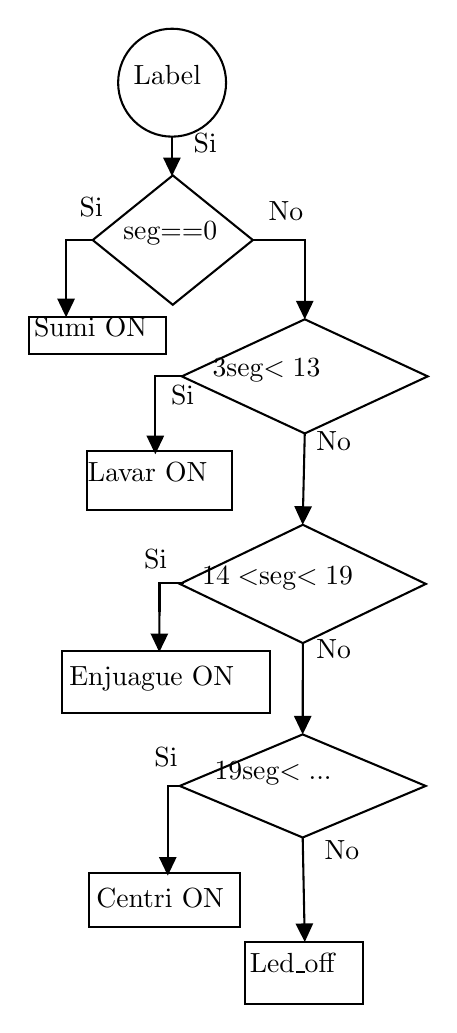
\begin{tikzpicture}[x=0.75pt,y=0.75pt,yscale=-1,xscale=1]
%uncomment if require: \path (0,501); %set diagram left start at 0, and has height of 501

%Flowchart: Connector [id:dp86445783611407] 
\draw   (280,41) .. controls (280,26.64) and (291.64,15) .. (306,15) .. controls (320.36,15) and (332,26.64) .. (332,41) .. controls (332,55.36) and (320.36,67) .. (306,67) .. controls (291.64,67) and (280,55.36) .. (280,41) -- cycle ;
%Flowchart: Decision [id:dp935312970889731] 
\draw   (306.33,85.67) -- (344.92,116.83) -- (306.33,148) -- (267.75,116.83) -- cycle ;
%Shape: Right Angle [id:dp07822486648512661] 
\draw   (267.75,116.83) -- (254.92,116.83) -- (254.92,128) ;
%Straight Lines [id:da37127883940863304] 
\draw    (254.92,128) -- (254.92,151) ;
\draw [shift={(254.92,154)}, rotate = 270] [fill={rgb, 255:red, 0; green, 0; blue, 0 }  ][line width=0.08]  [draw opacity=0] (8.93,-4.29) -- (0,0) -- (8.93,4.29) -- cycle    ;
%Flowchart: Process [id:dp4908952967414264] 
\draw   (236.92,154) -- (302.92,154) -- (302.92,171.81) -- (236.92,171.81) -- cycle ;
%Straight Lines [id:da7626068450578292] 
\draw    (369.92,129) -- (369.92,152) ;
\draw [shift={(369.92,155)}, rotate = 270] [fill={rgb, 255:red, 0; green, 0; blue, 0 }  ][line width=0.08]  [draw opacity=0] (8.93,-4.29) -- (0,0) -- (8.93,4.29) -- cycle    ;
%Shape: Right Angle [id:dp1235200916676118] 
\draw   (344.92,116.83) -- (369.92,116.83) -- (369.92,129) ;
%Flowchart: Decision [id:dp0636696577602811] 
\draw   (369.92,155) -- (429.17,182.5) -- (369.92,210) -- (310.67,182.5) -- cycle ;
%Shape: Right Angle [id:dp25067118553920165] 
\draw   (310.67,182.5) -- (297.92,182.5) -- (297.92,209) ;
%Straight Lines [id:da7947446829986125] 
\draw    (297.92,209) -- (297.92,217) ;
\draw [shift={(297.92,220)}, rotate = 270] [fill={rgb, 255:red, 0; green, 0; blue, 0 }  ][line width=0.08]  [draw opacity=0] (8.93,-4.29) -- (0,0) -- (8.93,4.29) -- cycle    ;
%Flowchart: Process [id:dp8895352375244476] 
\draw   (264.92,218.67) -- (334.92,218.67) -- (334.92,247) -- (264.92,247) -- cycle ;
%Straight Lines [id:da9249878842399695] 
\draw    (369.92,210) -- (368.98,251) ;
\draw [shift={(368.92,254)}, rotate = 271.3] [fill={rgb, 255:red, 0; green, 0; blue, 0 }  ][line width=0.08]  [draw opacity=0] (8.93,-4.29) -- (0,0) -- (8.93,4.29) -- cycle    ;
%Flowchart: Decision [id:dp027950767579304037] 
\draw   (369,254) -- (428.25,282.5) -- (369,311) -- (309.75,282.5) -- cycle ;
%Shape: Right Angle [id:dp7113899430080068] 
\draw   (311.75,282.17) -- (299.92,282.17) -- (299.92,296) ;
%Straight Lines [id:da6331255525268646] 
\draw    (299.92,296) -- (299.85,312.33) ;
\draw [shift={(299.83,315.33)}, rotate = 270.25] [fill={rgb, 255:red, 0; green, 0; blue, 0 }  ][line width=0.08]  [draw opacity=0] (8.93,-4.29) -- (0,0) -- (8.93,4.29) -- cycle    ;
%Flowchart: Process [id:dp31180552945320983] 
\draw   (253,314.67) -- (353,314.67) -- (353,344.67) -- (253,344.67) -- cycle ;
%Straight Lines [id:da1282233954801908] 
\draw    (369,311) -- (368.92,352) ;
\draw [shift={(368.92,355)}, rotate = 270.11] [fill={rgb, 255:red, 0; green, 0; blue, 0 }  ][line width=0.08]  [draw opacity=0] (8.93,-4.29) -- (0,0) -- (8.93,4.29) -- cycle    ;
%Flowchart: Decision [id:dp5974483452503938] 
\draw   (368.92,355) -- (428.17,379.83) -- (368.92,404.67) -- (309.67,379.83) -- cycle ;
%Shape: Right Angle [id:dp3217161793632042] 
\draw   (309.67,379.83) -- (303.92,379.83) -- (303.92,408) ;
%Straight Lines [id:da6569908124389181] 
\draw    (303.92,408) -- (303.92,420) ;
\draw [shift={(303.92,423)}, rotate = 270] [fill={rgb, 255:red, 0; green, 0; blue, 0 }  ][line width=0.08]  [draw opacity=0] (8.93,-4.29) -- (0,0) -- (8.93,4.29) -- cycle    ;
%Flowchart: Process [id:dp9233334167885809] 
\draw   (266,421.67) -- (338.92,421.67) -- (338.92,448) -- (266,448) -- cycle ;
%Straight Lines [id:da0014516432713123084] 
\draw    (368.92,404.67) -- (369.86,452) ;
\draw [shift={(369.92,455)}, rotate = 268.86] [fill={rgb, 255:red, 0; green, 0; blue, 0 }  ][line width=0.08]  [draw opacity=0] (8.93,-4.29) -- (0,0) -- (8.93,4.29) -- cycle    ;
%Straight Lines [id:da24463353428391343] 
\draw    (305.92,67) -- (305.92,83) ;
\draw [shift={(305.92,86)}, rotate = 270] [fill={rgb, 255:red, 0; green, 0; blue, 0 }  ][line width=0.08]  [draw opacity=0] (8.93,-4.29) -- (0,0) -- (8.93,4.29) -- cycle    ;
%Flowchart: Process [id:dp8528821341043025] 
\draw   (340.92,455) -- (397.92,455) -- (397.92,485) -- (340.92,485) -- cycle ;

% Text Node
\draw (286,31) node [anchor=north west][inner sep=0.75pt]   [align=left] {Label};
% Text Node
\draw (281,106.67) node [anchor=north west][inner sep=0.75pt]   [align=left] {seg==0};
% Text Node
\draw (238,152.5) node [anchor=north west][inner sep=0.75pt]   [align=left] {Sumi ON};
% Text Node
\draw (351,96.67) node [anchor=north west][inner sep=0.75pt]   [align=left] {No};
% Text Node
\draw (304,185.67) node [anchor=north west][inner sep=0.75pt]   [align=left] {Si};
% Text Node
\draw (260,94.67) node [anchor=north west][inner sep=0.75pt]   [align=left] {Si};
% Text Node
\draw (324,172.67) node [anchor=north west][inner sep=0.75pt]   [align=left] {$\displaystyle 3\leqslant $seg$\displaystyle < 13$};
% Text Node
\draw (255,222.67) node [anchor=north west][inner sep=0.75pt]   [align=left] { \ \ Lavar ON};
% Text Node
\draw (374,207.67) node [anchor=north west][inner sep=0.75pt]   [align=left] {No};
% Text Node
\draw (319,272.67) node [anchor=north west][inner sep=0.75pt]   [align=left] {$\displaystyle 14< $seg$\displaystyle < 19$};
% Text Node
\draw (255,320.67) node [anchor=north west][inner sep=0.75pt]   [align=left] {Enjuague ON};
% Text Node
\draw (291,264.67) node [anchor=north west][inner sep=0.75pt]   [align=left] {Si};
% Text Node
\draw (374,307.67) node [anchor=north west][inner sep=0.75pt]   [align=left] {No};
% Text Node
\draw (325,366.67) node [anchor=north west][inner sep=0.75pt]   [align=left] {$\displaystyle 19\leqslant $seg$\displaystyle < ...$};
% Text Node
\draw (268,427.67) node [anchor=north west][inner sep=0.75pt]   [align=left] {Centri ON};
% Text Node
\draw (296,359.67) node [anchor=north west][inner sep=0.75pt]   [align=left] {Si};
% Text Node
\draw (378,404.67) node [anchor=north west][inner sep=0.75pt]   [align=left] {No};
% Text Node
\draw (341.92,459) node [anchor=north west][inner sep=0.75pt]   [align=left] {Led\_off};
% Text Node
\draw (314.92,64) node [anchor=north west][inner sep=0.75pt]   [align=left] {Si};


\end{tikzpicture}


\caption{Conituación máquina de estados transición de LEDs.}
\label{sch3.1}
\end{figure}